% Requires in preamble:
% \usepackage{pgfplots}
% \pgfplotsset{compat=1.18}

\begin{figure}[htbp]
\centering
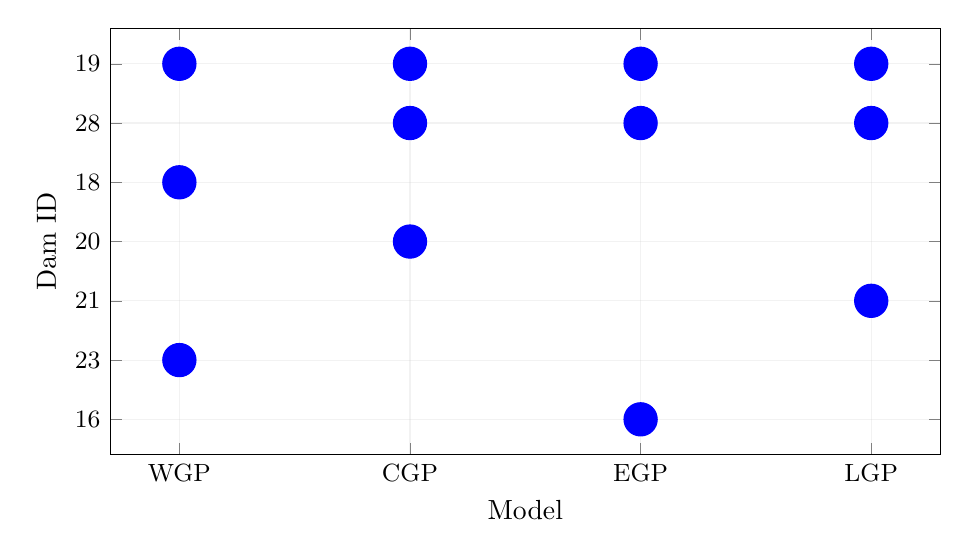
\begin{tikzpicture}
\begin{axis}[
  width=\textwidth,
  height=7cm,
  xlabel={Model},
  ylabel={Dam ID},
  xtick=data,
  ytick=data,
  symbolic x coords={WGP,CGP,EGP,LGP},
  symbolic y coords={19,28,18,20,21,23,16},
  y dir=reverse,
  grid=both,
  grid style={opacity=0.2},
  tick label style={font=\small},
]
\addplot[
  only marks,
  mark=*,
  mark size=6pt,
  color=blue,
  fill=blue
] coordinates {
  (WGP,19) (WGP,18) (WGP,23)
  (CGP,19) (CGP,20) (CGP,28)
  (EGP,19) (EGP,28) (EGP,16)
  (LGP,19) (LGP,28) (LGP,21)
};
\end{axis}
\end{tikzpicture}
\caption{Model–dam selection map for the four GP variants. Dam 19 is chosen by all four; Dam 28 by three (CGP, EGP, LGP); the others are singletons (WGP: 18, 23; CGP: 20; EGP: 16; LGP: 21).}
\label{fig:modelDamSelectionMap}
\end{figure}
